\documentclass[18pt]{beamer}
\usepackage[utf8]{inputenc} % for the umlauts

\beamertemplatenavigationsymbolsempty
%% SLIDE FORMAT

% use 'beamerthemekit' for standard 4:3 ratio
% for widescreen slides (16:9), use 'beamerthemekitwide'

\usepackage{templates/beamerthemekit}
% \usepackage{templates/beamerthemekitwide}

\setcounter{tocdepth}{1}

%% TITLE PICTURE

% if a custom picture is to be used on the title page, copy it into the 'logos'
% directory, in the line below, replace 'mypicture' with the 
% filename (without extension) and uncomment the following line
% (picture proportions: 63 : 20 for standard, 169 : 40 for wide
% *.eps format if you use latex+dvips+ps2pdf, 
% *.jpg/*.png/*.pdf if you use pdflatex)

%\titleimage{mypicture}

%% TikZ INTEGRATION

% use these packages for PCM symbols and UML classes
% \usepackage{templates/tikzkit}
% \usepackage{templates/tikzuml}

% the presentation starts here

\usepackage[absolute,overlay]{textpos}
%\usepackage[texcoord,grid,gridunit=mm,gridcolor=red, subgridcolor=green]{eso-pic}
\setbeamercovered{invisible}

\title[SWT1]{Softwaretechnik 1 - 1. Tutorium}
\subtitle{Tutorium 03}
\author{Felix Bachmann}
\date{15.05.2017}

\institute{KIT - Institut für Programmstrukturen und Datenorganisation (IPD)}

% Bibliography

\usepackage[citestyle=authoryear,bibstyle=numeric,hyperref,backend=biber]{biblatex}
\addbibresource{templates/example.bib}
\bibhang1em

\begin{document}

% change the following line to "ngerman" for German style date and logos
\selectlanguage{ngerman}

%title page
\begin{frame}
\titlepage
\end{frame}

%table of contents
\begin{frame}{Themenübersicht}
\tableofcontents
\end{frame}

\section{Organisatorisches}
	\subsection{Keine Lösungen ins Forum!}
	\begin{frame}
		\frametitle{Keine Lösungen ins Forum schreiben!}
		%TODO pic of censored forum thread \includegraphics[height=0.85\textheight]{}
	\end{frame}

\section{Wasserfallmodell}
	\subsection{Wasserfallmodell, ohne Grafik}
	\begin{frame}
		\frametitle{Wasserfallmodell}
		\begin{itemize}
			\item Was ist das? 
		\end{itemize}
	\end{frame}
	
	\subsection{Wasserfallmodell, mit Grafik}
	\begin{frame}
		\frametitle{Wasserfallmodell}
		dokumentengetriebenes Modell, das die (möglichen) Phasen der Softwareentwicklung beschreibt
		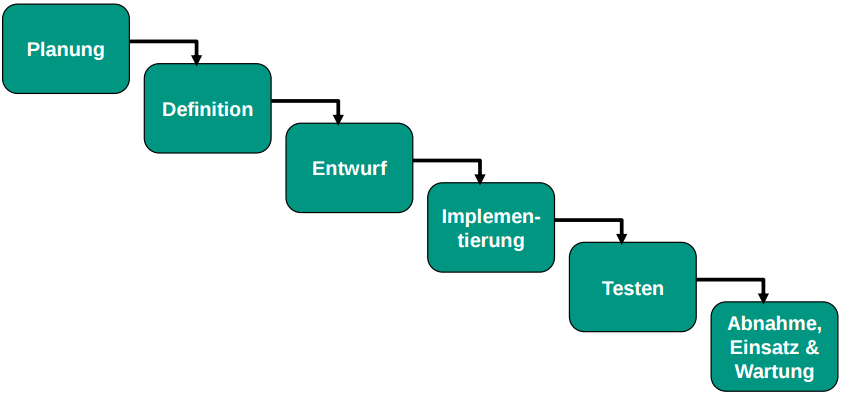
\includegraphics[scale=0.4]{./pics/tut1/waterfall_without-docs.png}
	\end{frame}
	
	\subsection{Wasserfallmodell, mit Grafik und Dokumenten}
	\begin{frame}
		\frametitle{Wasserfallmodell}
		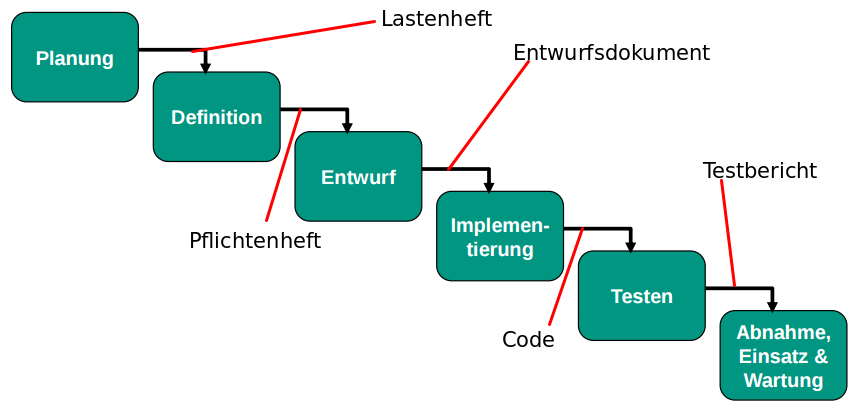
\includegraphics[scale=0.4]{./pics/tut1/waterfall_with-docs.png}
		Dokumente für das 2. ÜB: 
		\begin{itemize}
			\item Lastenheft
			\item Durchführbarkeitsuntersuchung (weiteres Artefakt der Planung)
		\end{itemize}
	\end{frame}

\section{Durchführbarkeitsuntersuchung}

\section{Lastenheft}

\section{Pflichtenheft}

\section{UML-Klassendiagramm}
		
\section{Tipps}
	\subsection{Tipps}
	\begin{frame}
		\frametitle{Tipps - 2. Übungsblatt}
		\begin{small}
			\begin{exampleblock}{Aufgabe 1}
				%TODO
			\end{exampleblock}
			\pause
			\begin{exampleblock}{Aufgabe 2}
				%TODO
			\end{exampleblock}
			\pause
			\begin{exampleblock}{Aufgabe 3}
				%TODO
			\end{exampleblock}
		\end{small}
	\end{frame}
	
	\subsection{Abgabe}
	\begin{frame}
		\frametitle{Denkt dran!}
		\begin{alertblock}{Abgabe}
			%TODO
		\end{alertblock}
	\end{frame}
		
	\begin{frame}
		\frametitle{Bis dann! (dann=15.05.17)}
		\centering
		%TODO comic \includegraphics[height=0.85\textheight]{}
	\end{frame}

\end{document}
